\documentclass[10pt,a4paper]{article}
\usepackage[utf8]{inputenc}
\usepackage[spanish]{babel}
\usepackage{graphicx}
\usepackage{subcaption}
\usepackage{fancyhdr}
\usepackage{amsmath}
\usepackage{amsfonts}
\usepackage{amssymb}
\usepackage{eurosym}
\usepackage{tikz}
\usetikzlibrary {arrows.meta}
%\usepackage[includehead=true,includefoot=true,portrait,top = 1cm]{geometry}
\usepackage[left=4cm,right=4cm,top=2cm,bottom=5cm]{geometry}
\graphicspath{{./FIGURAS/}}

%\fancyhf{}
\headsep = 2cm
\lhead{Nombre:}
%\lhead{{\huge\textbf{B}} Nombre:}
\chead{}
\rhead{
\includegraphics[scale=0.05]{gallinita.pdf}}
\lfoot{}
\cfoot{}
\rfoot{\today}
\newcommand{\valve}[3]{%
    \draw (#1,#2-.5) -- (#1,#2+.5) -- (#1+2,#2-.5) -- (#1+2,#2+0.5) -- cycle;
    \draw (#1+1,#2) -- (#1+1,#2+0.5);
    \draw (#1+0.75,#2+0.5) rectangle (#1+1.25,#2+0.7);
    \node at (#1+1,#2-1) {\bf #3};
}

\newcommand{\process}[3]{%
    \draw [rounded corners=2.5mm,fill=white, draw = black] (#1-1,#2-0.5) rectangle (#1+1,#2+2);
    \node at (#1,#2) {\bf #3};
}

\newcommand{\pump}[5]{%
        \filldraw [color=white,draw=black](#1,#2) circle (0.6);
        \draw[arrows = {-Latex[width'=5pt .5, length=10pt]}](#1,#2)--(#1+0.6,#2);
        \node at (#1+#3,#2+#4) {\bf #5};
}

\def\labelitemi{$\square$}
\begin{document}
\thispagestyle{fancy}

\section*{Exámen de Sistemas Dinámicos y Realimentación\footnote{Las respuestas pueden subirse al Campus Virtual en un \emph{live script}, pdf o similar, incluyendo los códigos utilizados. Si alguien prefiere entregar las explicaciones y deducciones en papel, también puede hacerlo.}.}

\section{Primer Parcial.}
\begin{enumerate}
\item Dos bloques de masa idéntica $m$ están unidos entre sí y a dos paredes opuestas mediante muelles de constante $k$. La figura muestra un esquema del sistema completo. Las líneas de puntos que unen los bloques representan los muelles.

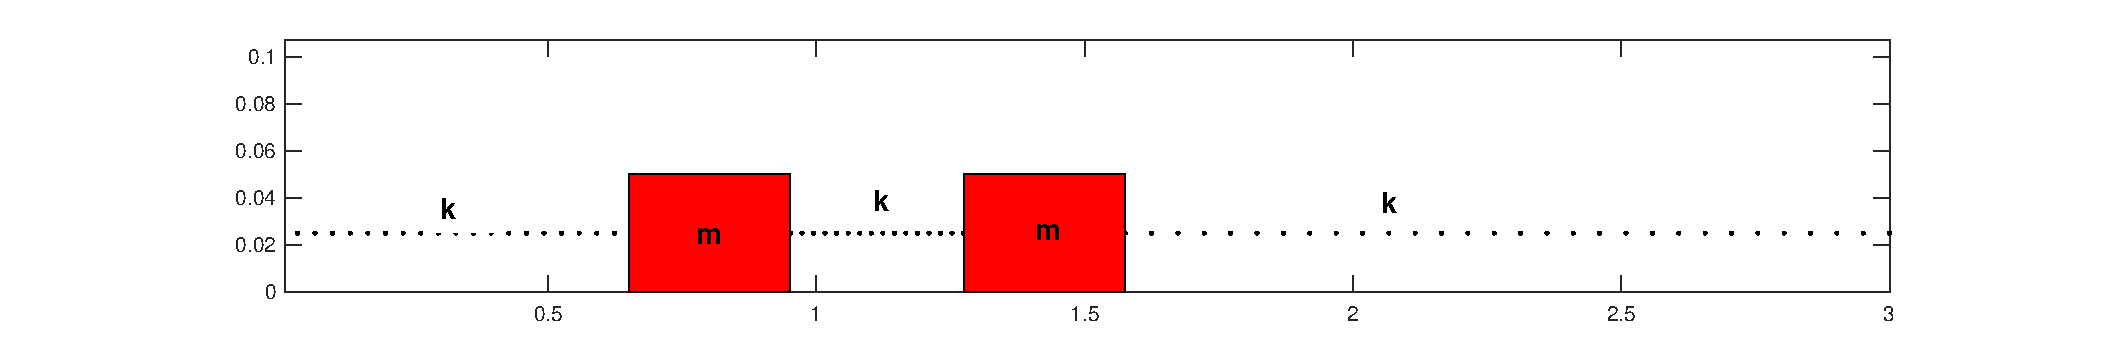
\includegraphics[width=\textwidth]{bloquecitos.eps}
Podemos obtener las ecuaciones del movimiento de los dos bloques en función de su desplazamiento desde su posición de equilibrio:
\begin{align*}
m\frac{d^2\Delta_1}{dt^2} &= -2k\cdot \Delta_1 +k\cdot \Delta_2 -\mu\frac{d\Delta_1}{dt}+F(t)\\
m\frac{d^2\Delta_2}{dt^2} &= -2k\cdot \Delta_2 +k\cdot \Delta_1 -\mu\frac{d\Delta_2}{dt}
\end{align*}

donde $\Delta_1$ y $\Delta_2$ son los desplazamientos de los bloques respecto a su posición de equilibrio y $\mu$ es un coeficiente de fricción igual para ambos bloques. Además, suponemos que es posible ejercer una fuerza externa sobre uno de los bloques, (bloque 1), pero no sobre el otro.
\begin{enumerate}
\item (1 punto) Describe el sistema mediante variables de estado de modo que $x_1=\Delta_1$, $x_2 =\Delta_2$, $x_3=\dot{\Delta}_1$, $x_4=\dot{\Delta}_2$.
Considera además que la única salida del sistema es el desplazamiento del bloque 2.  
\item \label{b} (1 punto) Comprueba que el sistema es controlable y diseña un sistema de estabilización por realimentación de estados --supón que ambos son accesibles-- de modo que los autovalores estén situados en $[-2, -2, -5, -5]$. Compara la respuesta del sistema en lazo abierto con la del sistema realimentado, suponiendo una entrada nula y condiciones iniciales $x_1=-0.5$, $x_2=0.7$, $x_3=0.2$, $x_4=0.3$. Emplea para los parámetros  $m= 1$, $k=3$ y $\mu=1$. Indica y justifica las principales diferencias. Comprueba que las posiciones que se obtienen son coherentes en ambos casos con el sistema (los bloques no chocan entre sí ni con las paredes). 

\item \label{c} (1.5 puntos) Comprueba que no es posible emplear control integral para situar a la vez ambos bloques en posiciones arbitrarias. Demuestra que sí es posible situar al menos el bloque del que se conoce  la posición. Añade al sistema de control diseñado en el apartado (\ref{b}) control integral, coloca el autovalor de la acción integral en $-5$ y emplealo para desplazar el bloque $2$ una distancia $x_2 = 0.35$ de su posición de equilibrio. Muestra gráficamente los resultados.


\item (1.5 puntos) Diseña un estimador de modo que sus autovalores estén desplazados cuatro unidades hacia a la izquierda respecto a los polos del sistema. Emplea el estimador para realimentar y controlar el sistema. Repite el calculo realizado en el apartado (\ref{c}) considera nulas las condiciones iniciales del estimador $\hat{x}_i=0$. ¿Sería posible controlar en la realidad este sistema sin el estimador? Razona la respuesta.

\end{enumerate}
\end{enumerate}

\section{Segundo Parcial}
\begin{enumerate}
\item Dado el sistema\footnote{\textbf{Si estás haciendo el final, contesta solo a esta pregunta.}},
\begin{equation}\label{eq1}
\begin{split}
\dot x_1 = x_1(x_1^2 + x_2^2 -1) -x_2\\
\dot x_2 = x_1 + x_2(x_1^2+x_2^2-1)
\end{split}
\end{equation}
\begin{enumerate}
\item (1 punto) Obtener los puntos de equilibrio del sistema. Linealizar en torno a ellos y discutir su estabilidad.
\item \label{apb} (2 puntos)  Emplea el criterio de estabilidad de Lyapunov del sistema linealizado, para obtener un función de Lyapunov y empleala para  estudiar la estabilidad del sistema no lineal.

\item (2 puntos) Resuelve numéricamente la ecuación (\ref{eq1}), Para distintos valores de las condiciones iniciales, y obtén un diagrama de fases del sistema. Comprueba que los resultados son coherentes con el análisis realizado en los apartados anteriores.
\end{enumerate}
\item Si multiplicamos por $-1$ ambos términos de la ecuación (\ref{eq1}), obtenemos el sistema:
\begin{equation}\label{eq2}
\begin{split}
\dot x_1 = -x_1(x_1^2 + x_2^2 -1) + x_2\\
\dot x_2 = -x_1 - x_2(x_1^2+x_2^2-1)
\end{split}
\end{equation}
\begin{enumerate}
\item (2.5 puntos) Estudia la estabilidad de los puntos de equilibrio del sistema, empleando la misma función de Lyapunov obtenida en el apartado \ref{apb}. ¿Es posible sacar alguna conclusión sobre la estabilidad del sistema?
\item (2.5 puntos) Resuelve numéricamente la ecuación (\ref{eq2}), Para distintos valores de las condiciones iniciales, y obtén un diagrama de fases del sistema. Comprueba que los resultados son coherentes con el análisis realizado en el apartado anterior. ¿Se puede establecer alguna relación entre los sistemas de los dos ejercicios?
\end{enumerate}
\end{enumerate}

\end{document}
